% !TEX root =  paper.tex
\section{Introduction}\label{sec:introduction}

% introduction to E2E test automation
Test automation techniques are used to enable the end-to-end (E2E) functional testing of web applications~\cite{DBLP:journals/ac/TonellaRM14}. 
In this context, the tester assumes the role of the end user and verifies the correct functioning of the application under test (AUT) by means of automated test scripts. Such scripts automate the set of manual operations that the end user performs on the web application GUI (e.g., delivering events with clicks, or filling in forms), and can run fast in a unattended mode. This makes them appealing in modern software development, where the ability to react fast to ever-changing requirements is essential. For this reason, test automation techniques are often used in agile or continuous integration (CI) environments where new test cases are being developed and added to existing test suites in parallel with the development of the software itself, and across a wide range of testing tasks such as regression, system and UI testing~\cite{STVR:STVR121,Fewster,Ramler:2006:EPT:1138929.1138946,Nguyen2014,7381848}.

% the problem

Despite their wide adoption, E2E test automation tools bring the problem of maintaining test scripts as software evolves. Changes as simple as repositioning GUI elements on the page or altering the selections in a drop-down list can cause the test to halt or behave improperly. 
In the literature, instances of these problems are known as \textit{test breakages}: a test breakage is defined as the event that occur when the test raises exceptions or errors that do not pertain to the presence of a bug or a malfunction of the application under test~\cite{Daniel:2011:AGR:2002931.2002937,Daniel:2009:RSR:1747491.1747538,Daniel:2010:TRU:1831708.1831734,Hammoudi-2016-ICST}. 
This is different from cases in which test cases \textit{fail}, that is, raise exceptions which signal the presence of one or more bugs in the production code. In this latter case, the developer is required to correct the application whereas in the former case, the tester is required to fix the tests. %, that are no longer synchronized with the AUT.

% existing work

Repairing tests is an activity that typically requires testers to inspect the GUI, or replay a portion of test scenario, in order to detect the root cause behind the breakage. The situation is complicated by the fact that breakages do not always occur at the precise point in which the test execution's stops, but rather at some later point.
% and handle the breakages that propagate throughout the test's execution~\cite{Hammoudi-2016-ICST}.

%Current techniques rely on the assumption that the repair has always to be triggered at the point in which the test stops, which makes it impossible to handle such propagated breakages~\cite{Hammoudi-2016-ICST}.

%While prior work has investigated the testware evolution problem~\cite{2016-leotta-Advances,2014-leotta-WoSAR,2015-leotta-ICST,Thummalapenta:2013:ECT:2486788.2486926,Yandrapally:2014:RTA:2610384.2610390,Choudhary:2011:WWA:2002931.2002935,Hammoudi-2016-FSE}, none comprehensively focuses on the specific difficulties of \textit{detection and repair of breakages} in web tests. 
%Existing web test repair techniques~\cite{Choudhary:2011:WWA:2002931.2002935,Hammoudi-2016-FSE,2015-leotta-ICST} are, in many cases, either unable to correct breakages, or do so by producing a great number of false positives. 
%%
%Moreover, due to their DOM-narrowness, none of which is designed to consider visual aspects of the AUT, they fail to enable testers to perform effective root cause analysis for a given breakage. 
None of the existing web test repair techniques~\cite{Choudhary:2011:WWA:2002931.2002935,Hammoudi-2016-FSE,2015-leotta-ICST} is designed to consider visual aspects of the AUT. Thereby such solutions are, in many cases, either unable to correct breakages, or do so by producing a great number of false positives. 

% our proposal

%For the scope of this paper, we present a new holistic approach to  web applications testing that considers both DOM-based and visual characteristics of the AUT in order to support \textit{automated repair of breakages in E2E web test cases}. 
For the scope of this paper, we propose \tool, a new generation algorithm that leverages the information given by the visual execution of the tests, along with computer vision and crawling techniques, to support \textit{automated repair of breakages in E2E web test cases}. 

%\begin{figure*}[t]
%\centering
%\begin{subfigure}{.20\linewidth}
%\centering
%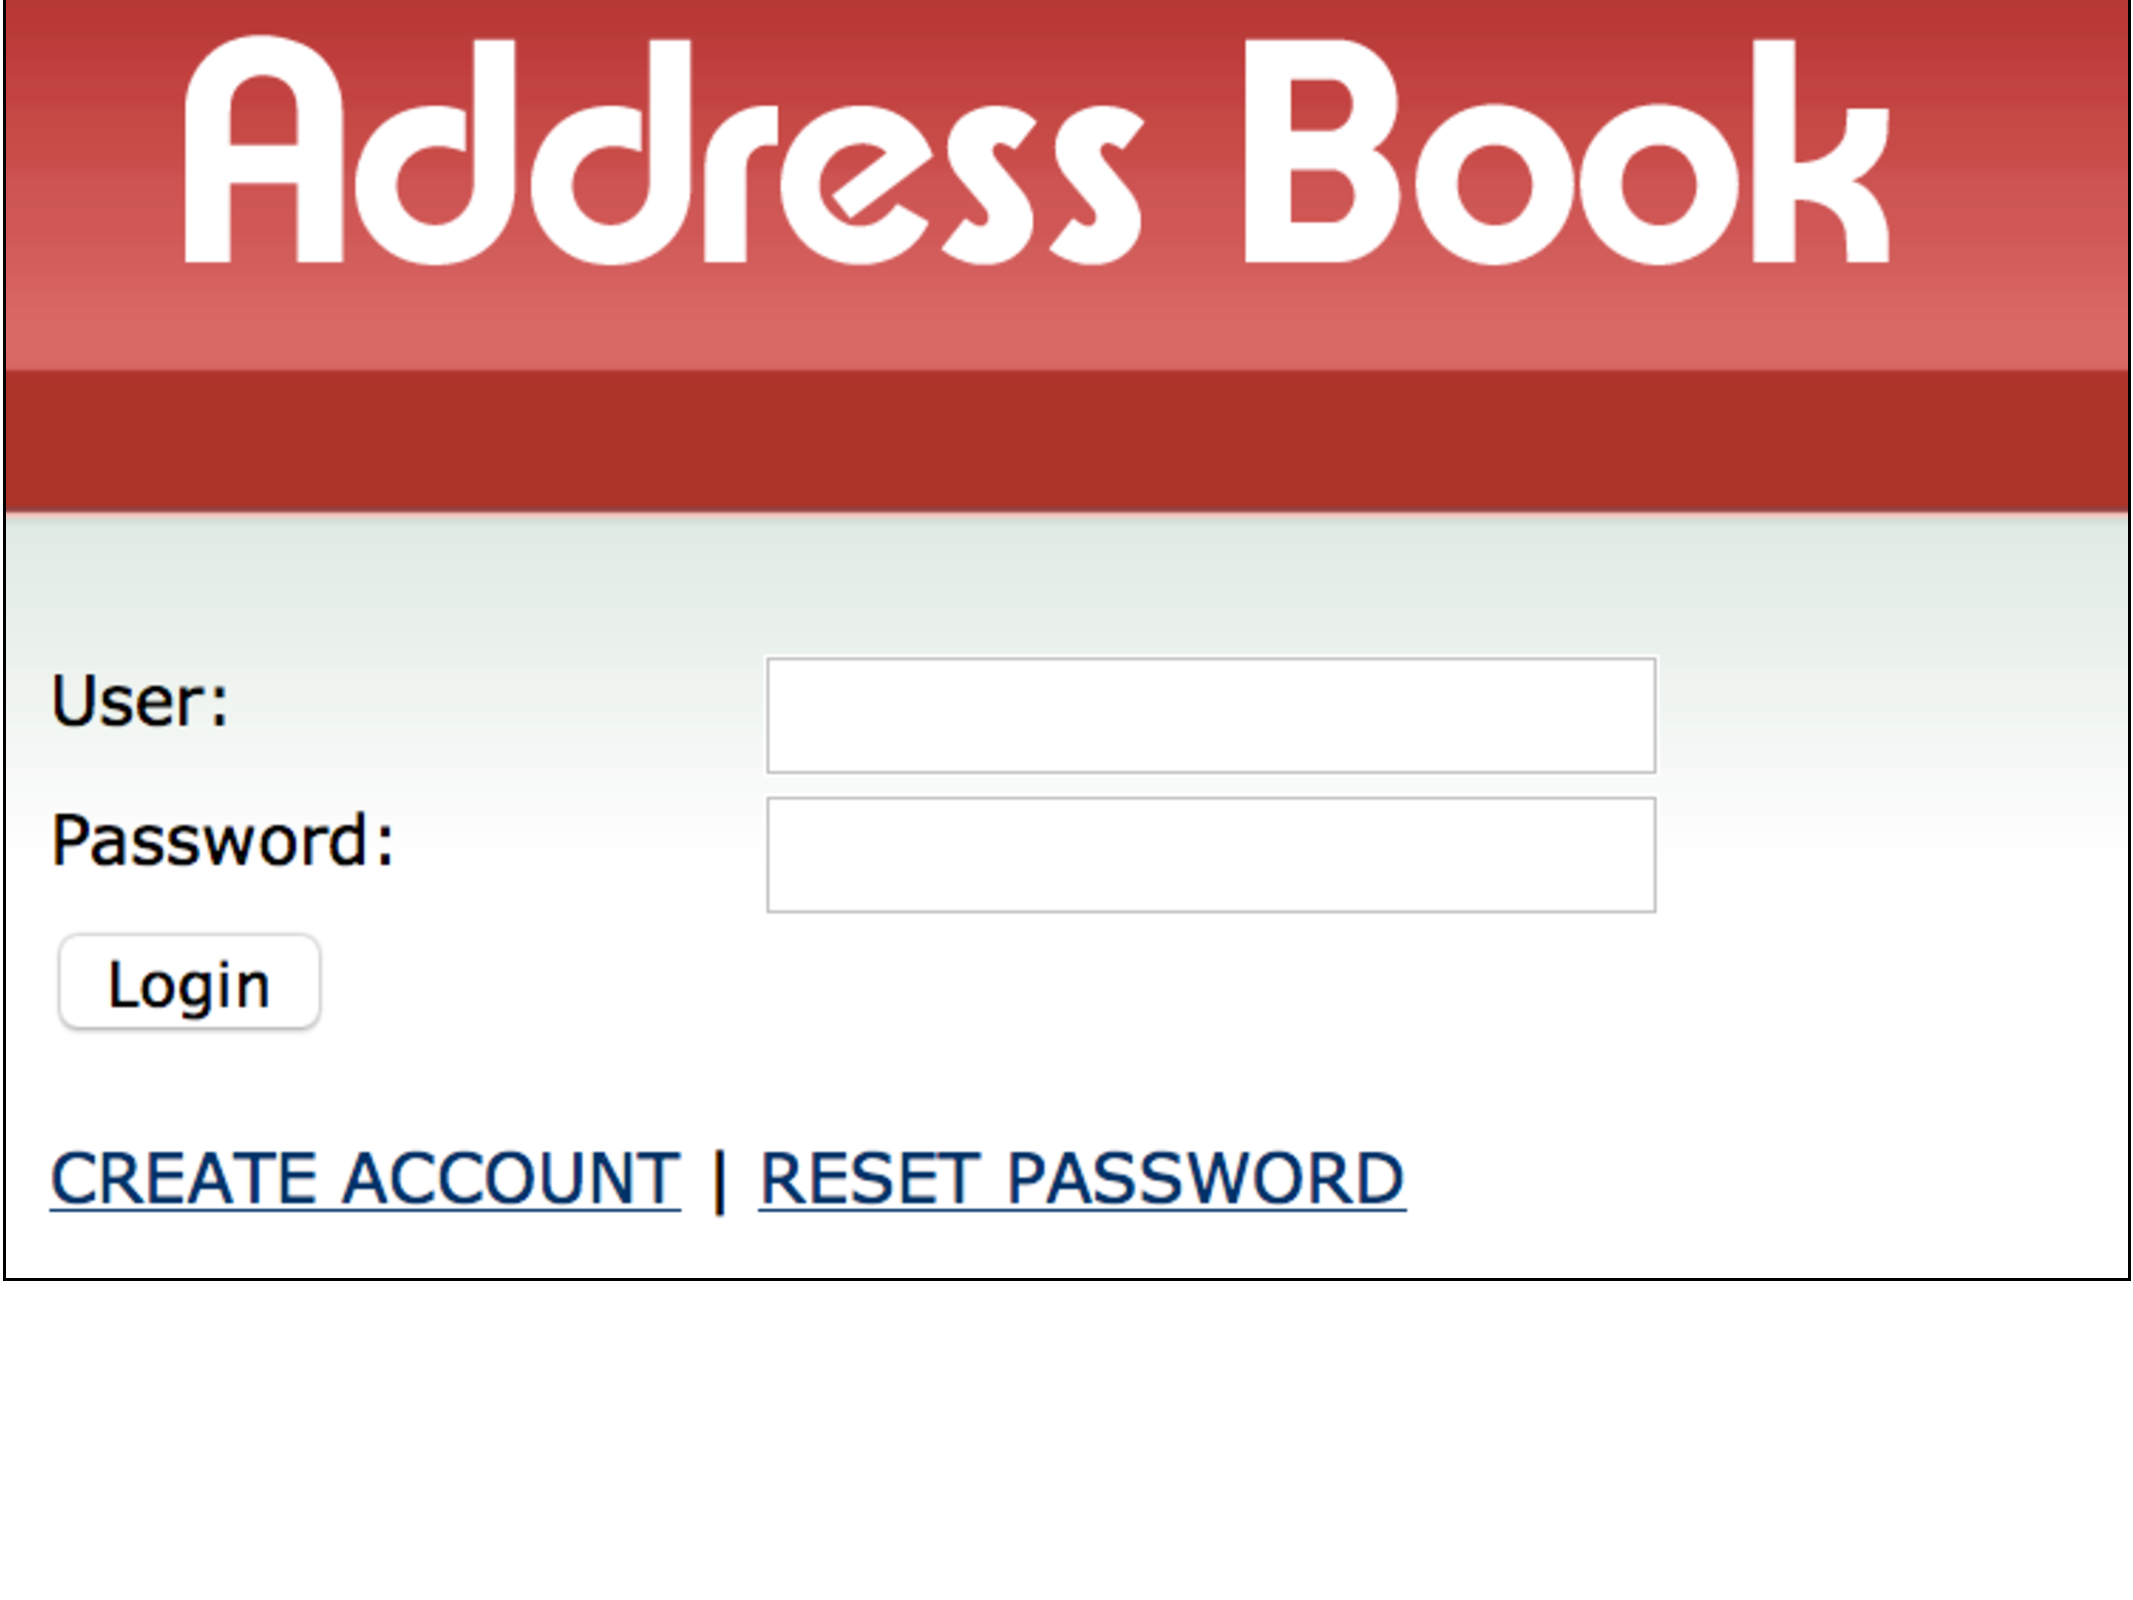
\includegraphics[trim=0cm 5.3cm 0.1cm 0.1cm, clip=true, scale=0.107]{images/ab1.pdf}
%\caption{\emph{Login page.}}
%\label{fig:ab-back-a} 
%\end{subfigure}
%\quad
%\begin{subfigure}{.25\linewidth}
%\centering
%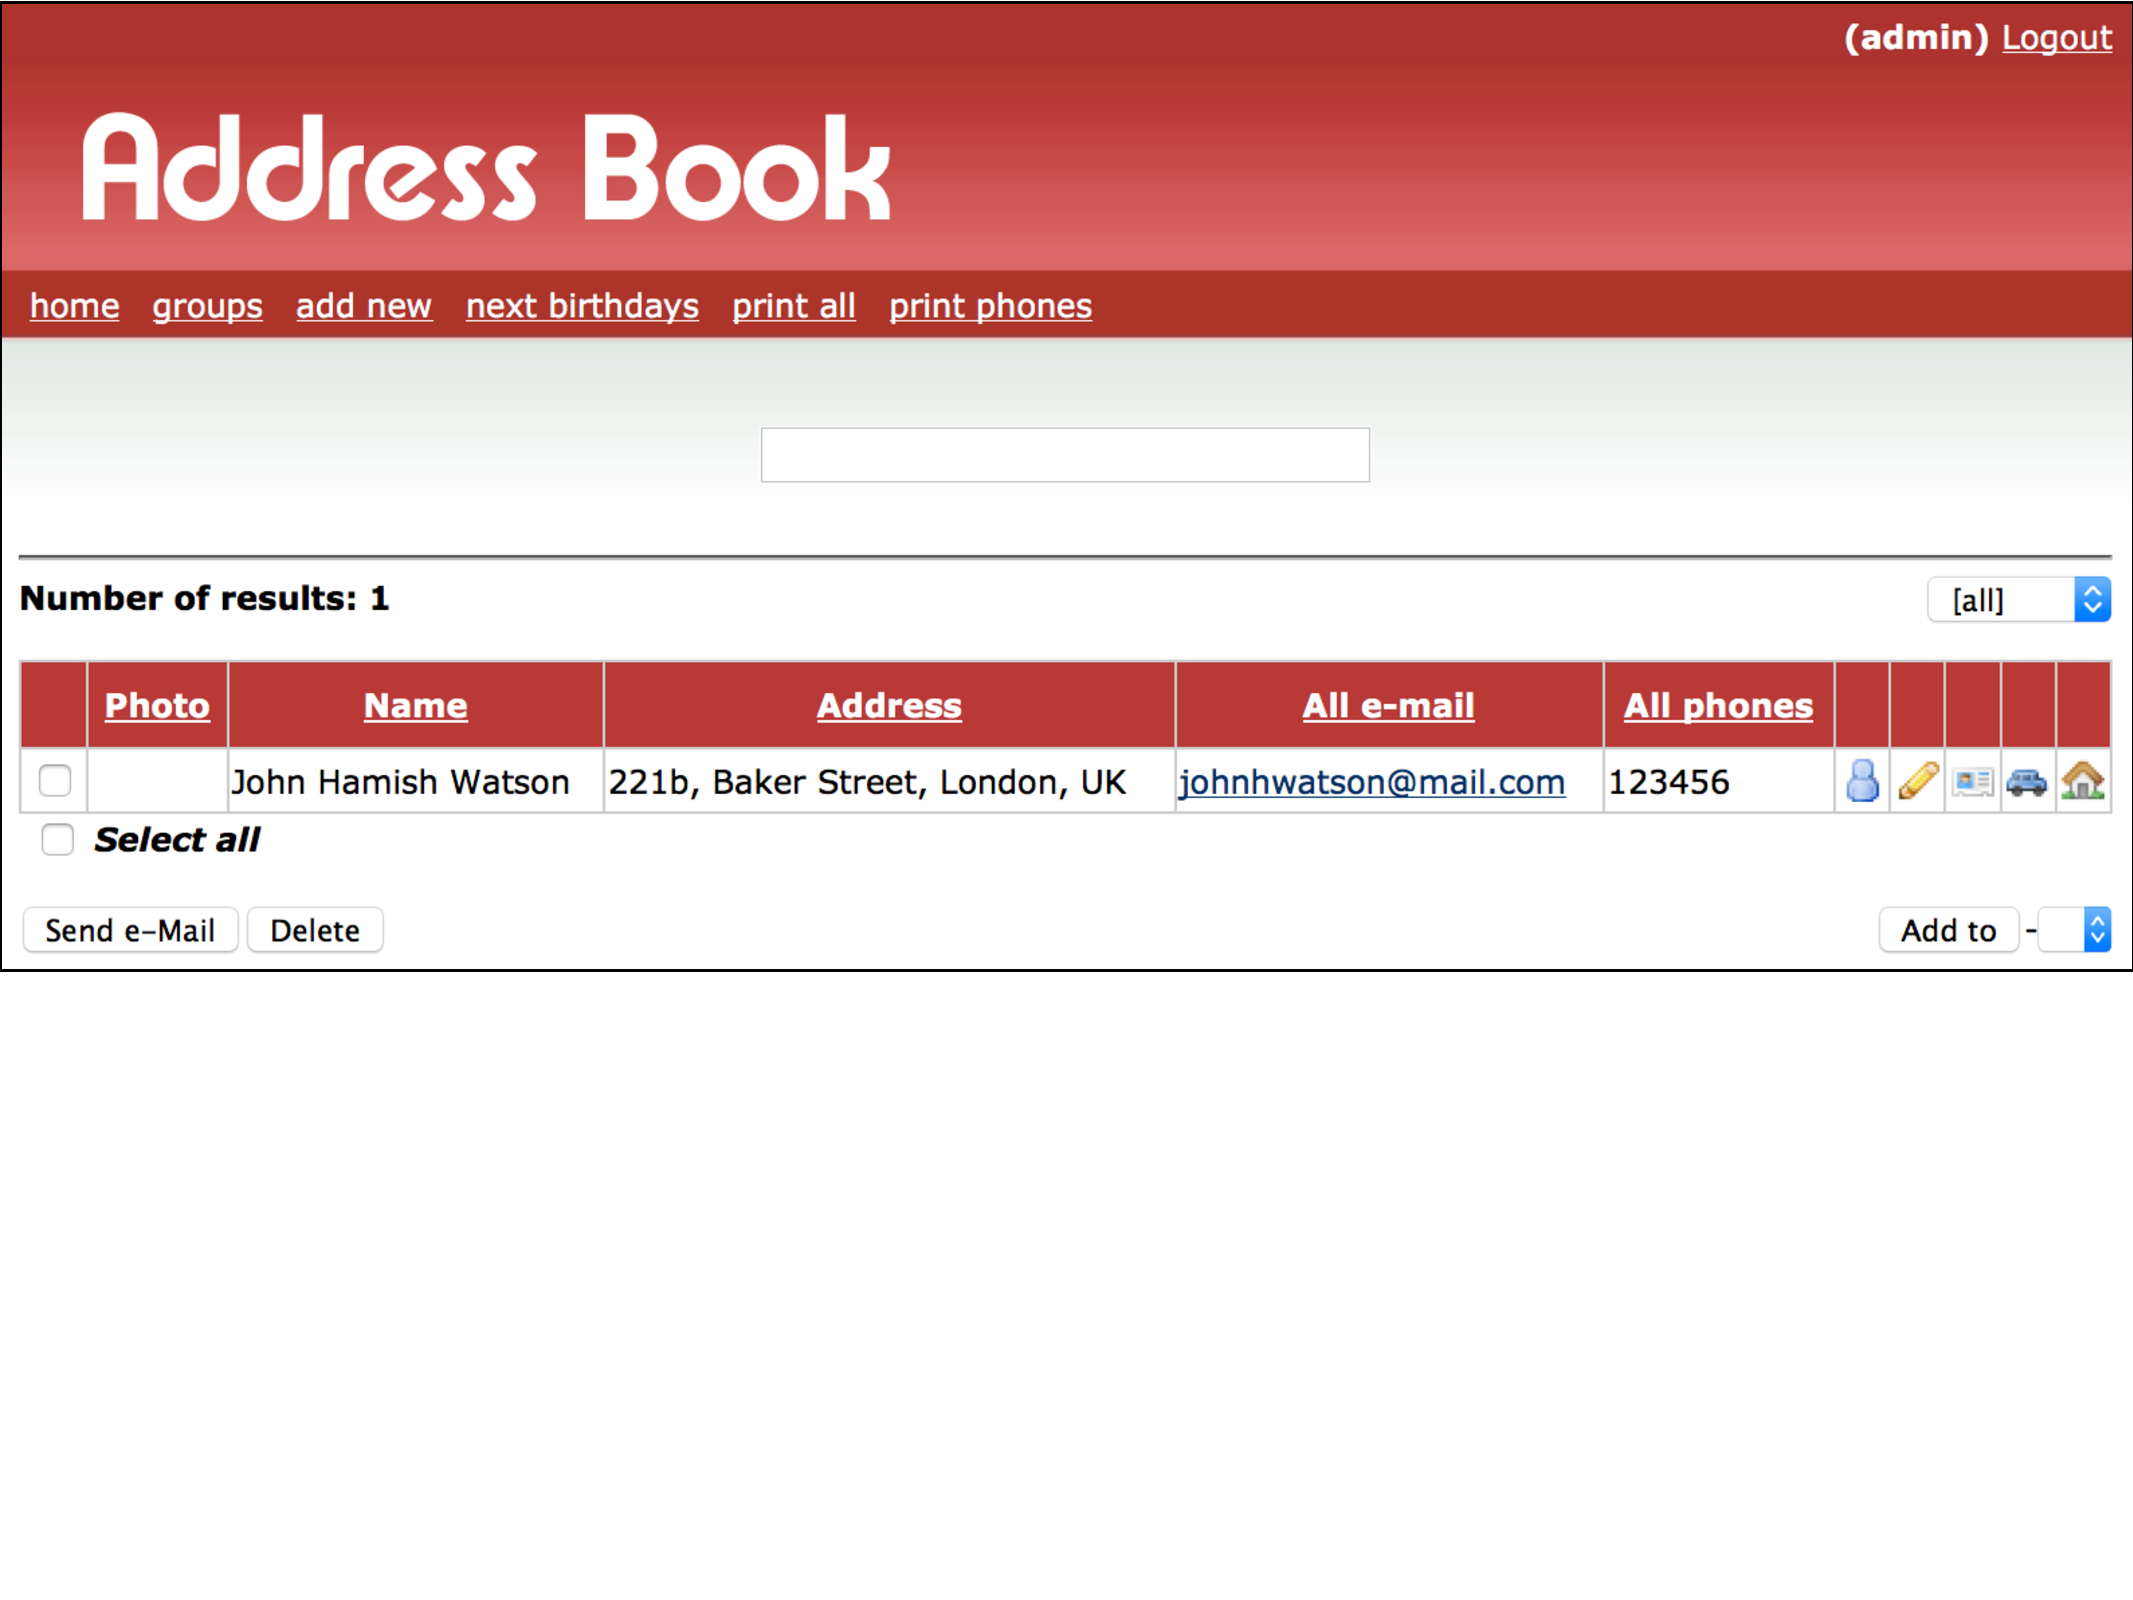
\includegraphics[trim=0cm 10.5cm 0cm 0cm, clip=true, scale=0.141]{images/ab2.pdf}
%\caption{\emph{Home page.}}
%\label{fig:ab-back-b} 
%\end{subfigure}
%\qquad
%\begin{subfigure}{.25\linewidth}
%\centering
%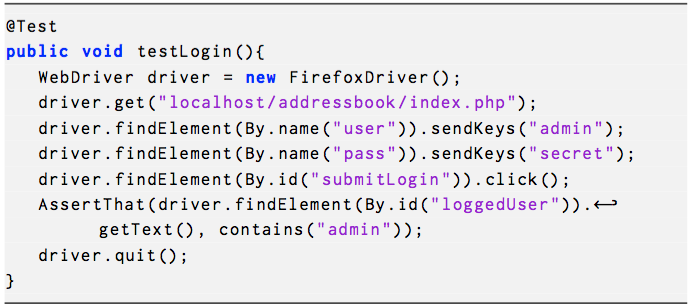
\includegraphics[trim=0cm 0cm 2cm 0cm, clip=true, scale=0.22]{images/test.png}
%\caption{\emph{DOM-based test.}}
%\label{fig:ab-back-c} 
%\end{subfigure}
%\quad
%\begin{subfigure}{.20\linewidth}
%\centering
%\fbox{
%{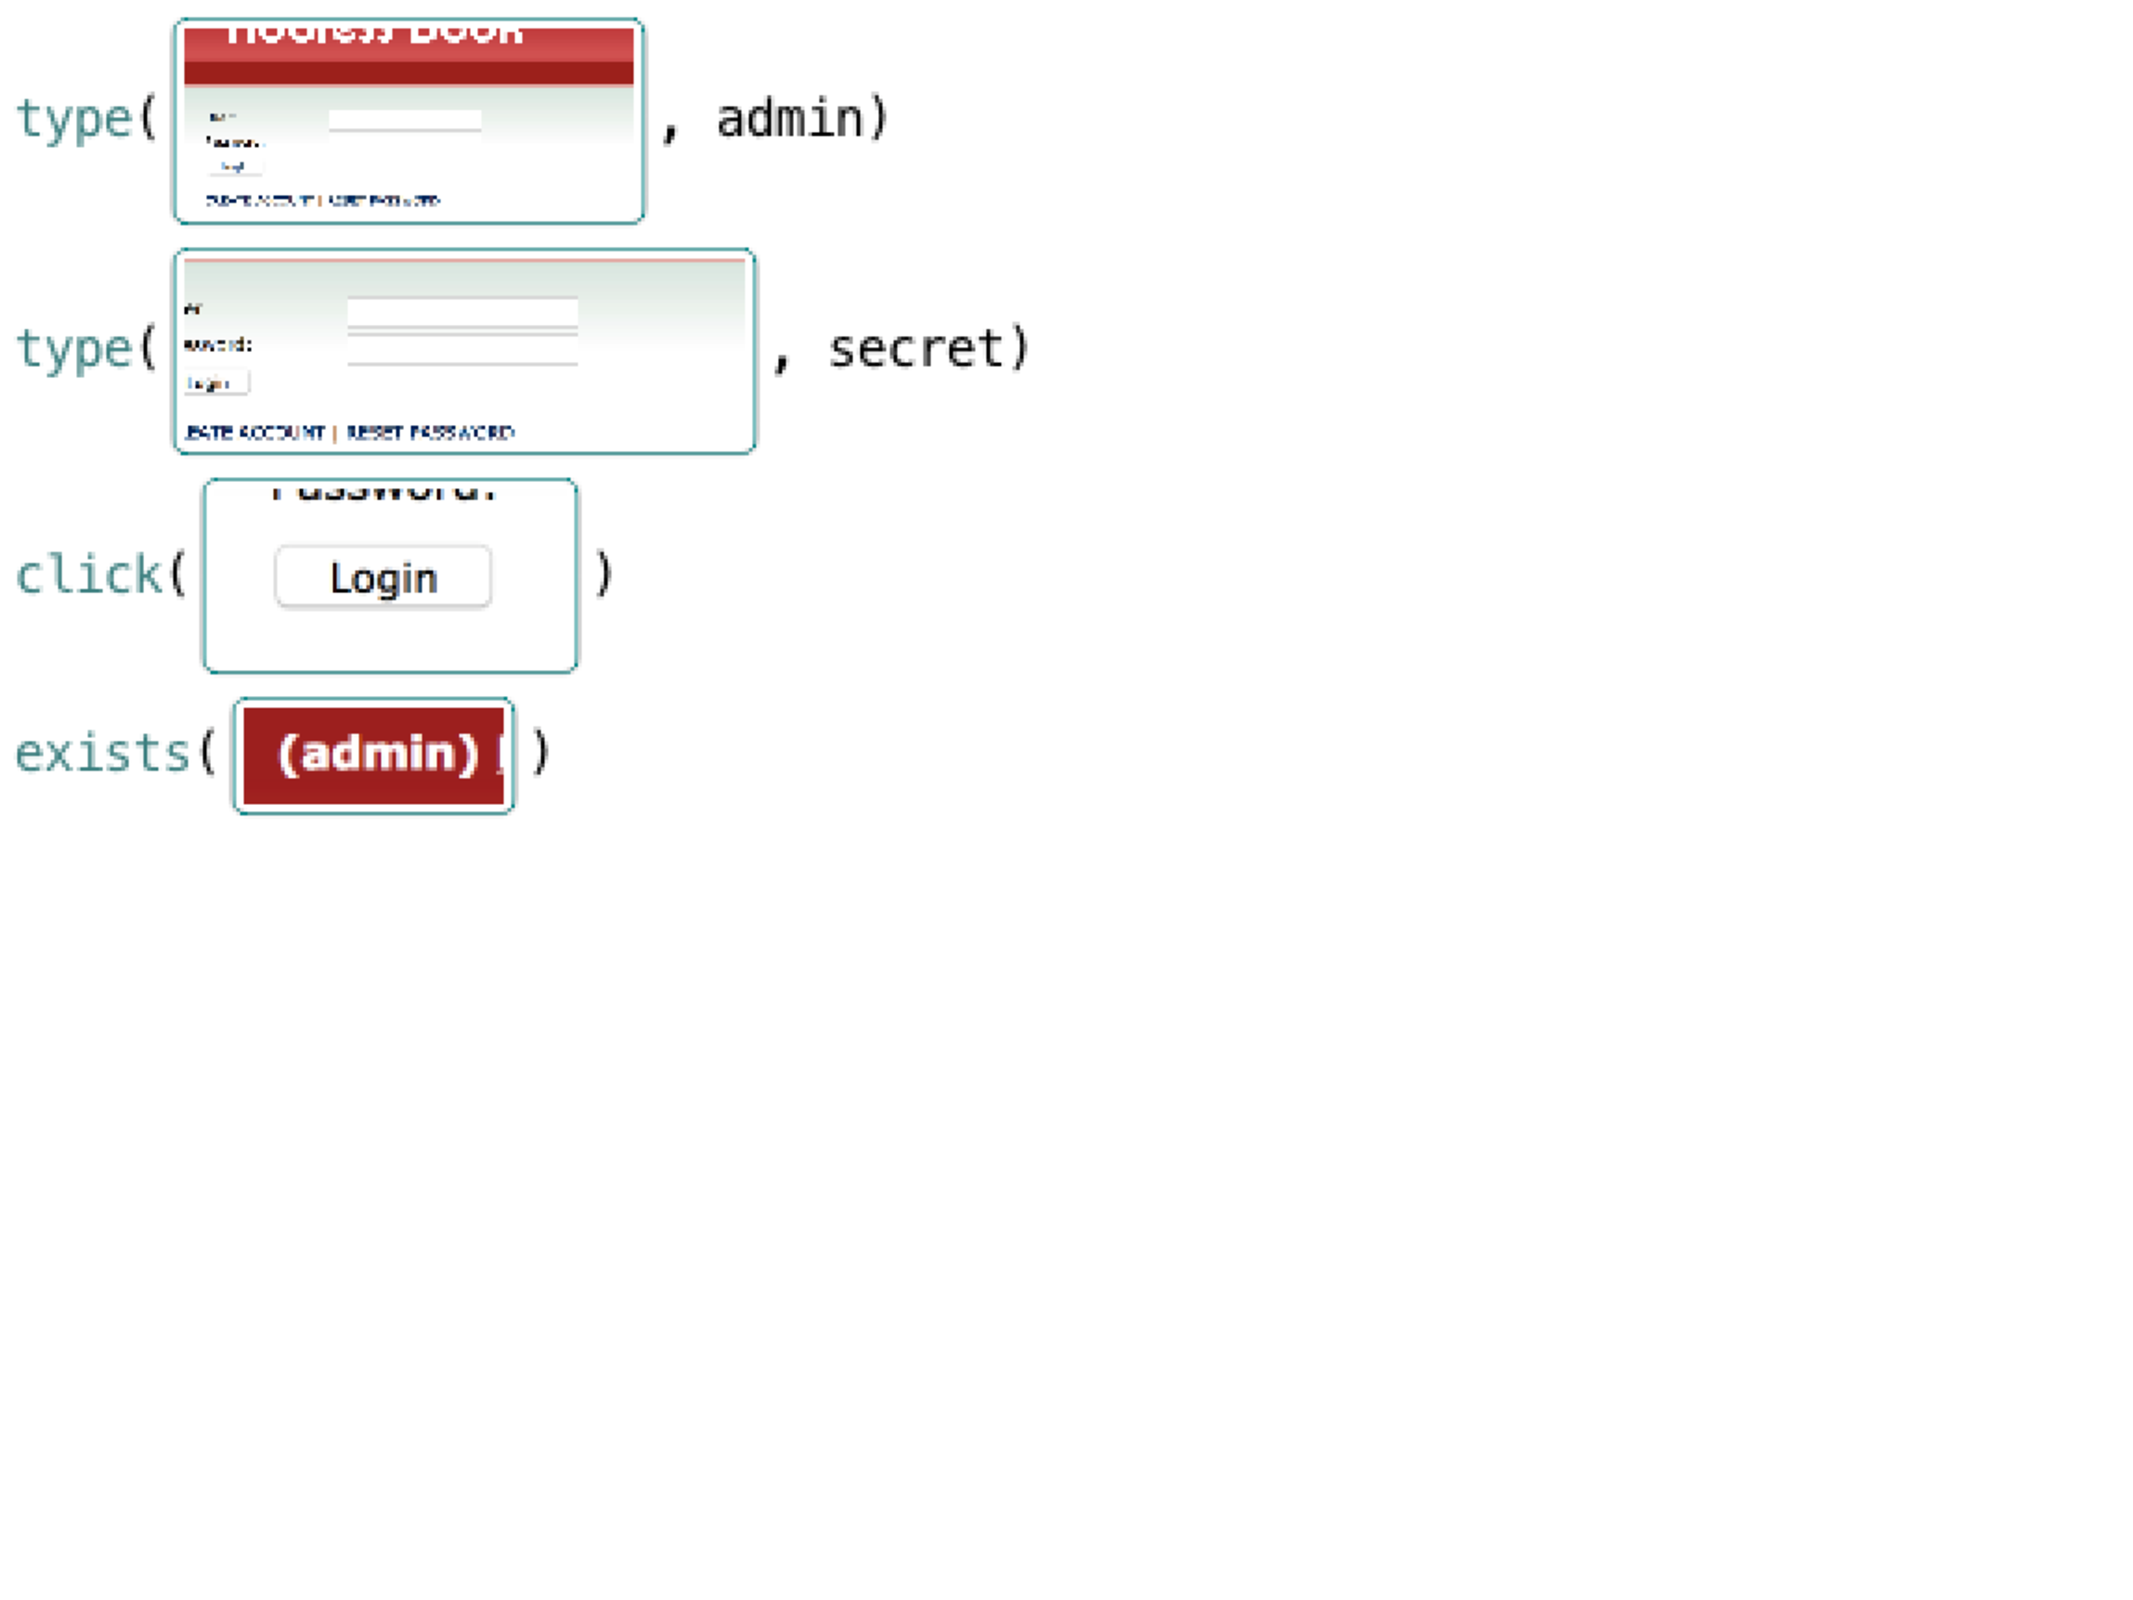
\includegraphics[trim=0.1cm 13cm 19cm 0.1cm, clip=true, scale=0.15]{images/sikuli-s.pdf}}
%}
%\caption{\emph{Visual test.}}
%\label{fig:ab-back-d} 
%\end{subfigure}
%\caption{AddressBook web application, and examples of DOM-based and visual automated test cases. \andrea{sync the web pages images with the other figures}}
%\label{fig:ab-back}
%\end{figure*}


The key idea behind the development of \tool is that the manual actions and reasoning that a tester does while searching for candidate repairs can be automated to a large extent by using differential testing, crawling, and computer vision. 
\tool maintains the visual snapshots of the correct execution of the test cases. When such tests are replayed on the new version of the AUT, \tool uses snapshots of the web elements visual appearance to validate the feasibility of each statement prior to their execution (\textit{online monitoring}). If \tool detects that a breakage will occur, then a series of repair techniques are triggered on the fly, to correct the breakage before executing it (\textit{self-repair}).

\tool is also able to handle complex breakage scenarios, such as those that break the test's workflow (e.g., when elements are removed from the web pages, or a page is added), using an automatic local visual-based crawl exploration.

We evaluated the capabilities of \tool in catching regressions on 2672 test cases spanning 82 releases for four real-world web applications. \tool was able to repair up to 81\% of the total number of breakages. 

This paper makes the following contributions.
\begin{itemize}
\item A repair-oriented taxonomy of test breakages in web applications.
\item An algorithm for verifying each executing test step and correct them should a breakage occur. 
\item An implementation 
\item An empirical evaluation 
\end{itemize}








